\section{Auswertung}
\todo[inline, color=red]{Vera}
\begin{figure}[H]
	
\includegraphics[width=\textwidth]{Images/Auswertung/Testbild1/SourceImage with PointPairs_onlydiffs.jpg}
	\caption{Differenzen zwischen den idealen und realen Stützpunkten.}
	\label{fig:diffsResult}
\end{figure}

\begin{figure}[H]
	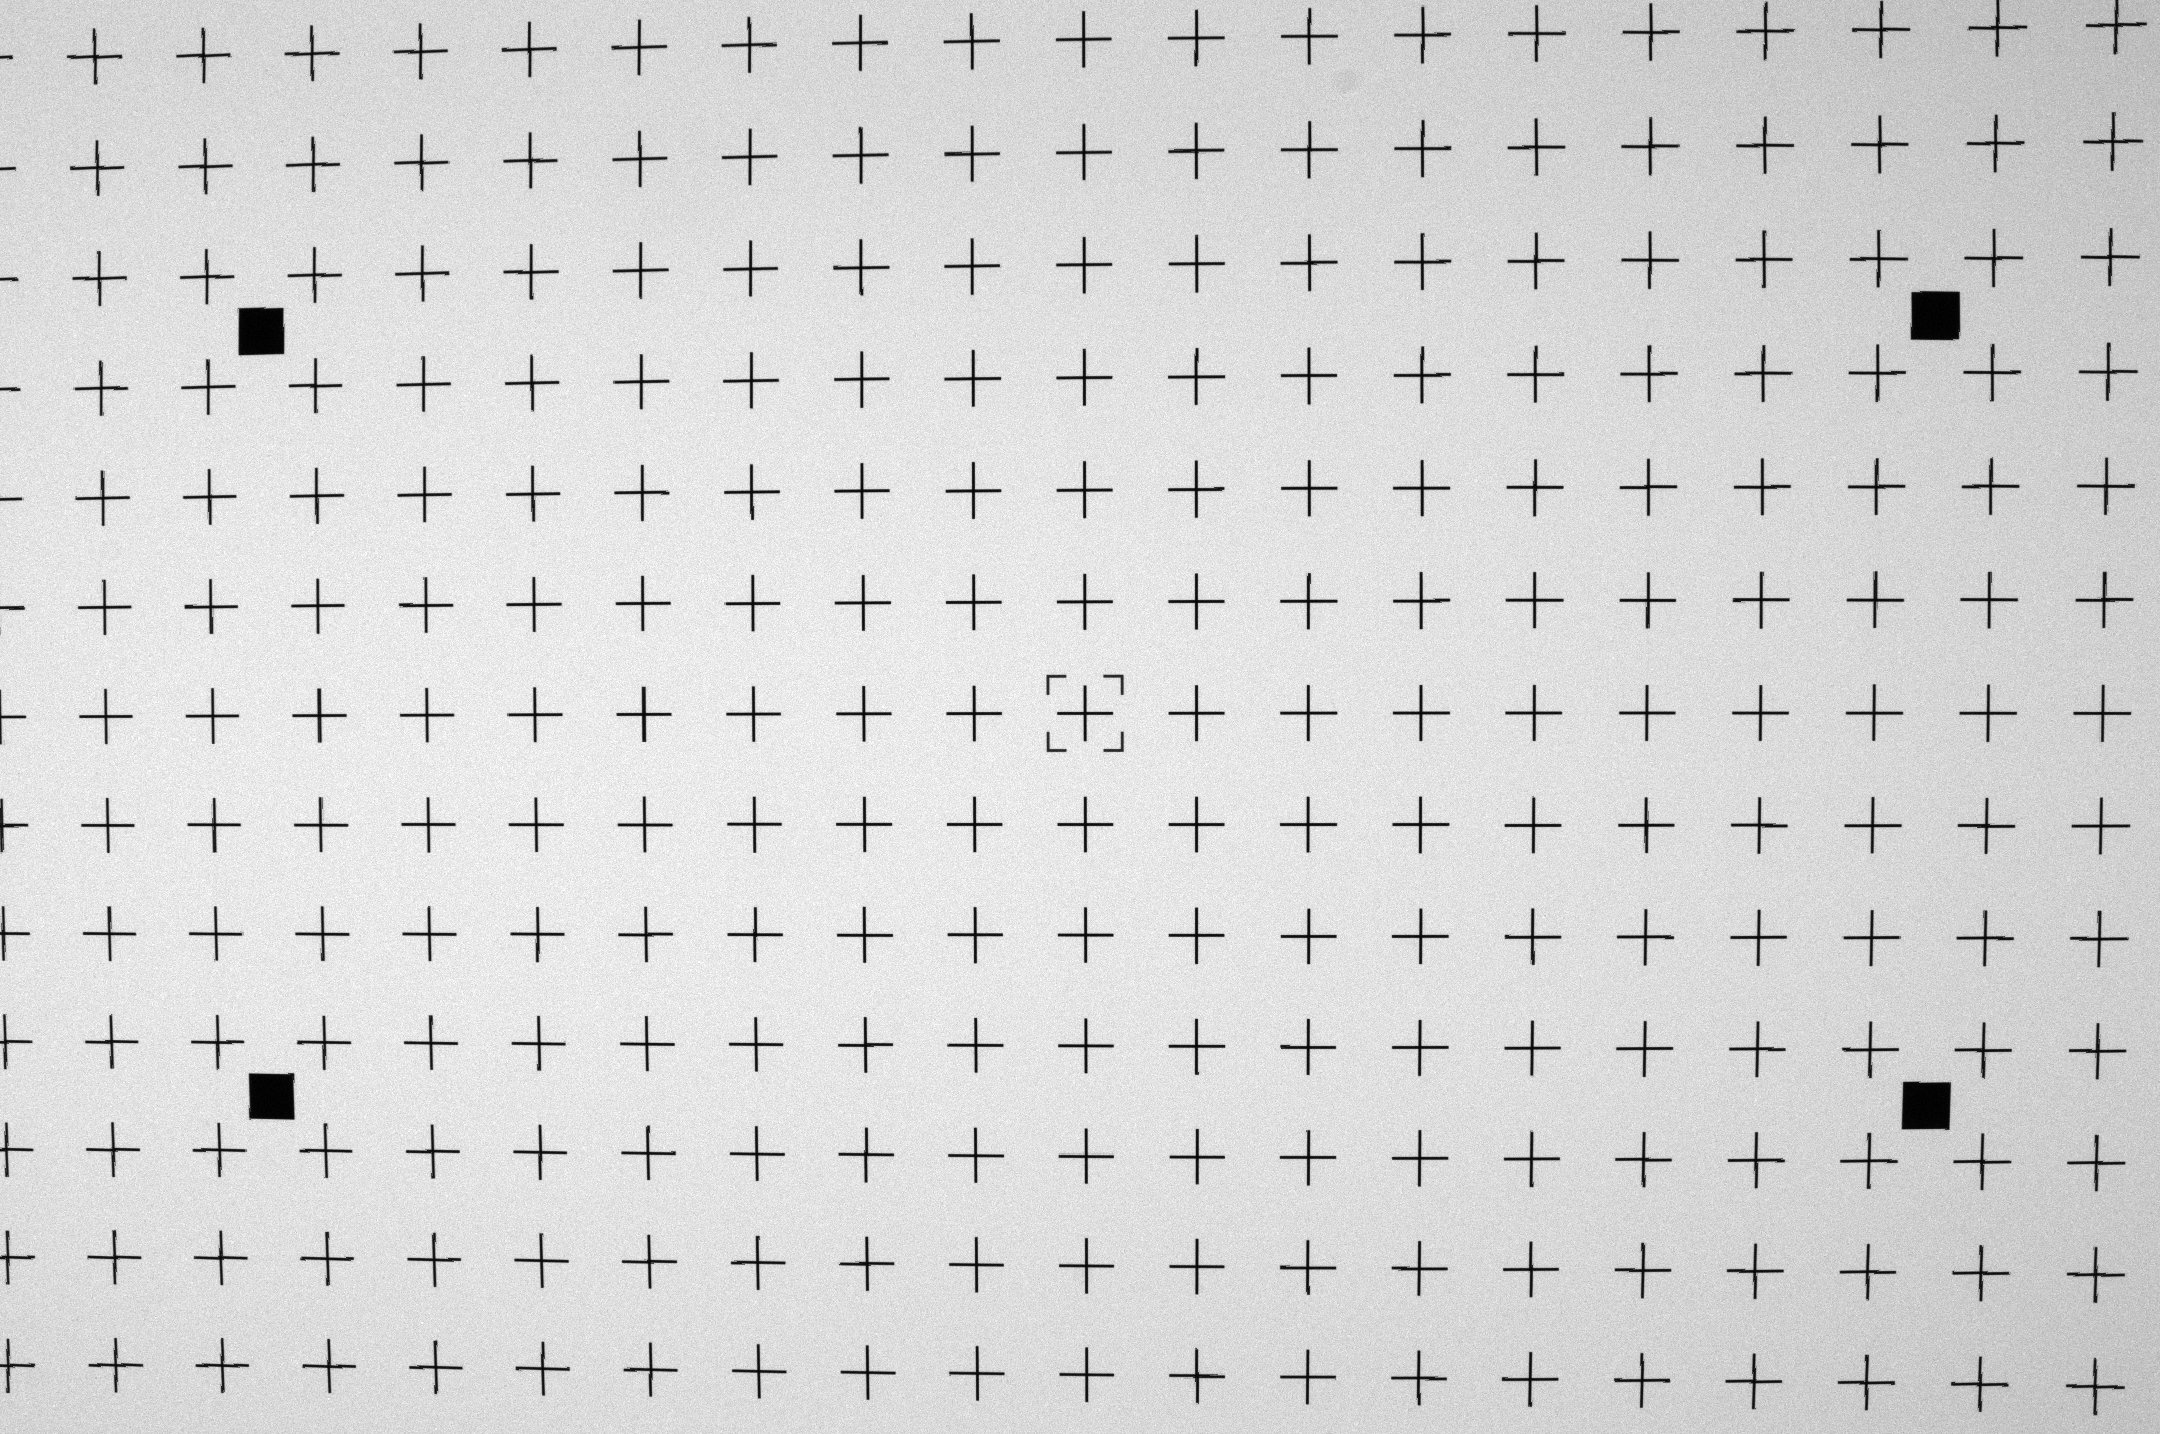
\includegraphics[width=\textwidth]{Images/Auswertung/Testbild1/Radial.jpg}
	\caption{Resultat der Radialen Entzerrrung}
	\label{fig:Ergebnis}
\end{figure}

\begin{figure}[H]
	
\includegraphics[width=\textwidth]{Images/Auswertung/Testbild1/Radial_onlydiffs.jpg}
	\caption{Differenzen zwischen den idealen und transformierten Stützpunkten.}
	\label{fig:diffsResult}
\end{figure}


